
\begin{frame}
	\frametitle{Piecewise Constant Method: Donor-Cell Advection}
	
	\begin{columns}
		\column{0.6\textwidth}
			Assume cell state within cell is constant.
			
			For $u = 1$:
			\begin{align*}
			\rho_i ^{n+1} &= \rho_i^{n} + 
			\frac{\Delta t}{\Delta x} (f_{i-\half}^{n+\half} - f_{i+\half}^{n+\half} )\\
			f_{i\pm\half}^{n+1} &= u_{i\pm\half}\quad \rho_{i - \half \pm \half}
			\end{align*}
			
			First order accurate in time and space.
			
		\column{.4\textwidth}
			\centering
			\includegraphics[width=\textwidth]{images/donorcell.png}
			\tiny{
				Image adapted from ``Lecture Numerical Fluid Dynamics'', Lecture given by C.P. Dullemond and H.H. Wang at Heidelberg University, 2009
			}
		
	\end{columns}
\end{frame}	






\begin{frame}
	\vspace{10pt}
	\begin{columns}
		\column{.33\textwidth}
			\centering
			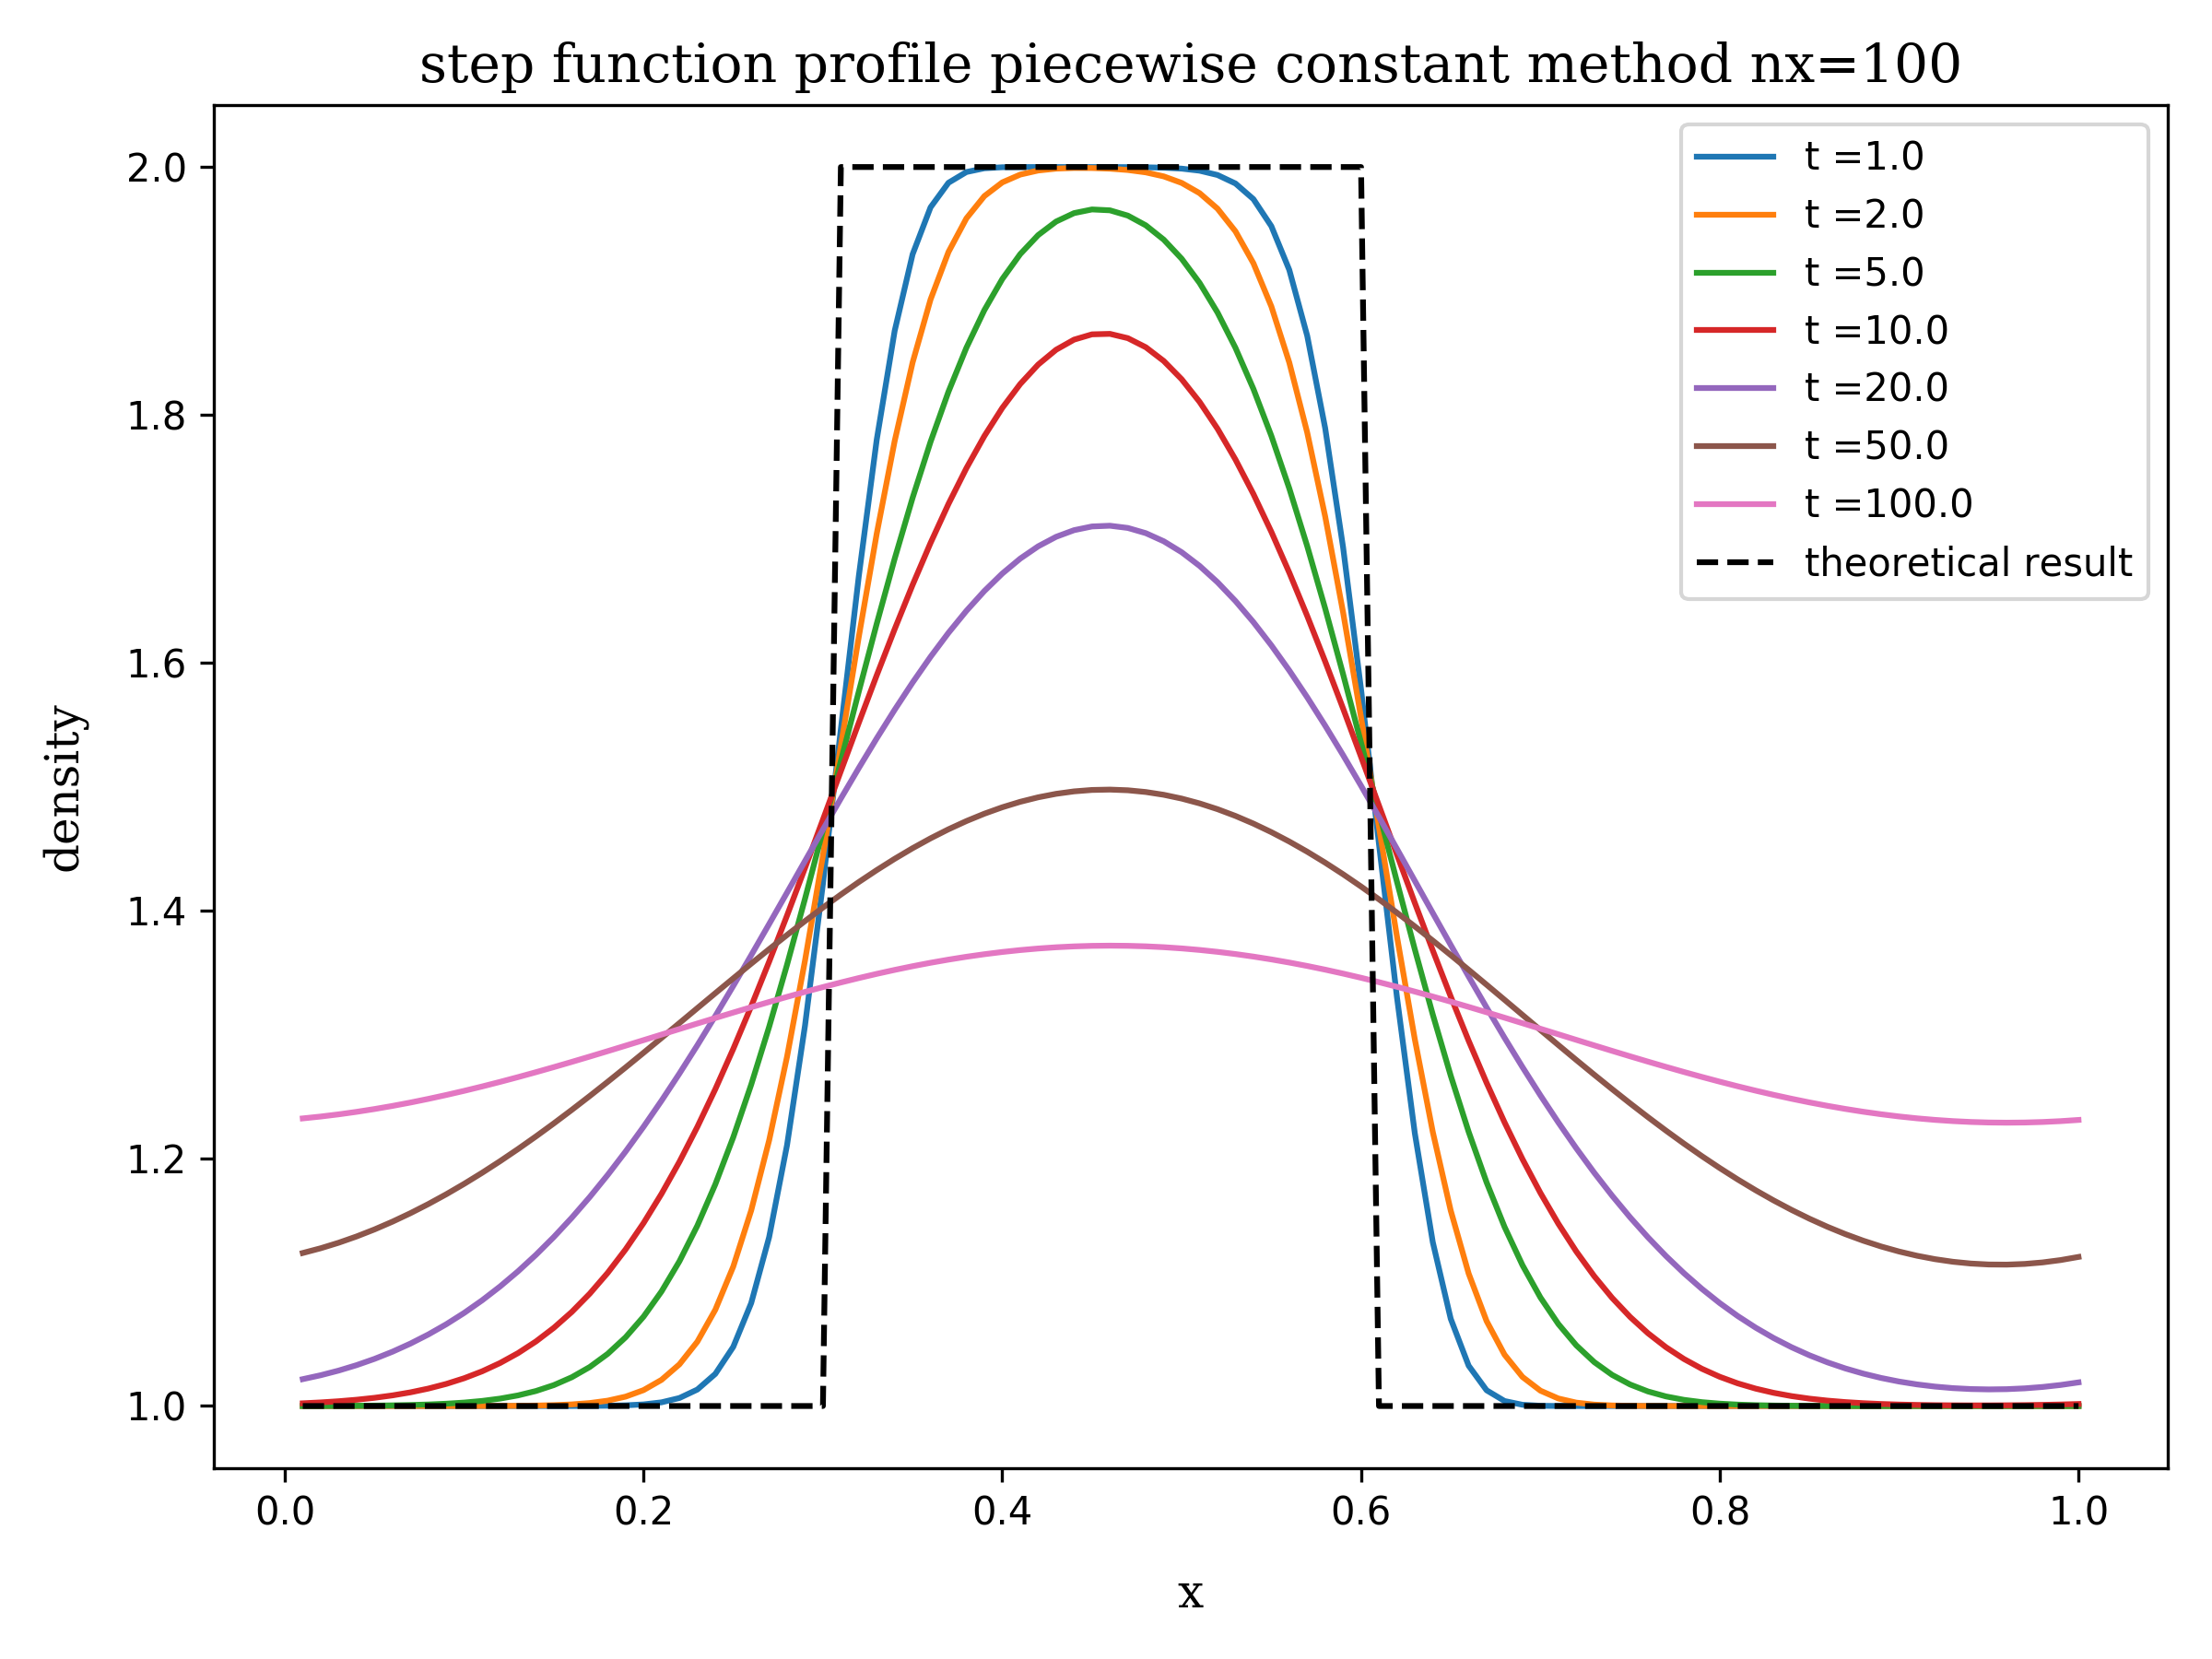
\includegraphics[height=.33\textheight]{../results/1D/pwconst/nx=100/plot_advection_step_function_pwconst_nx=100.png}\\
			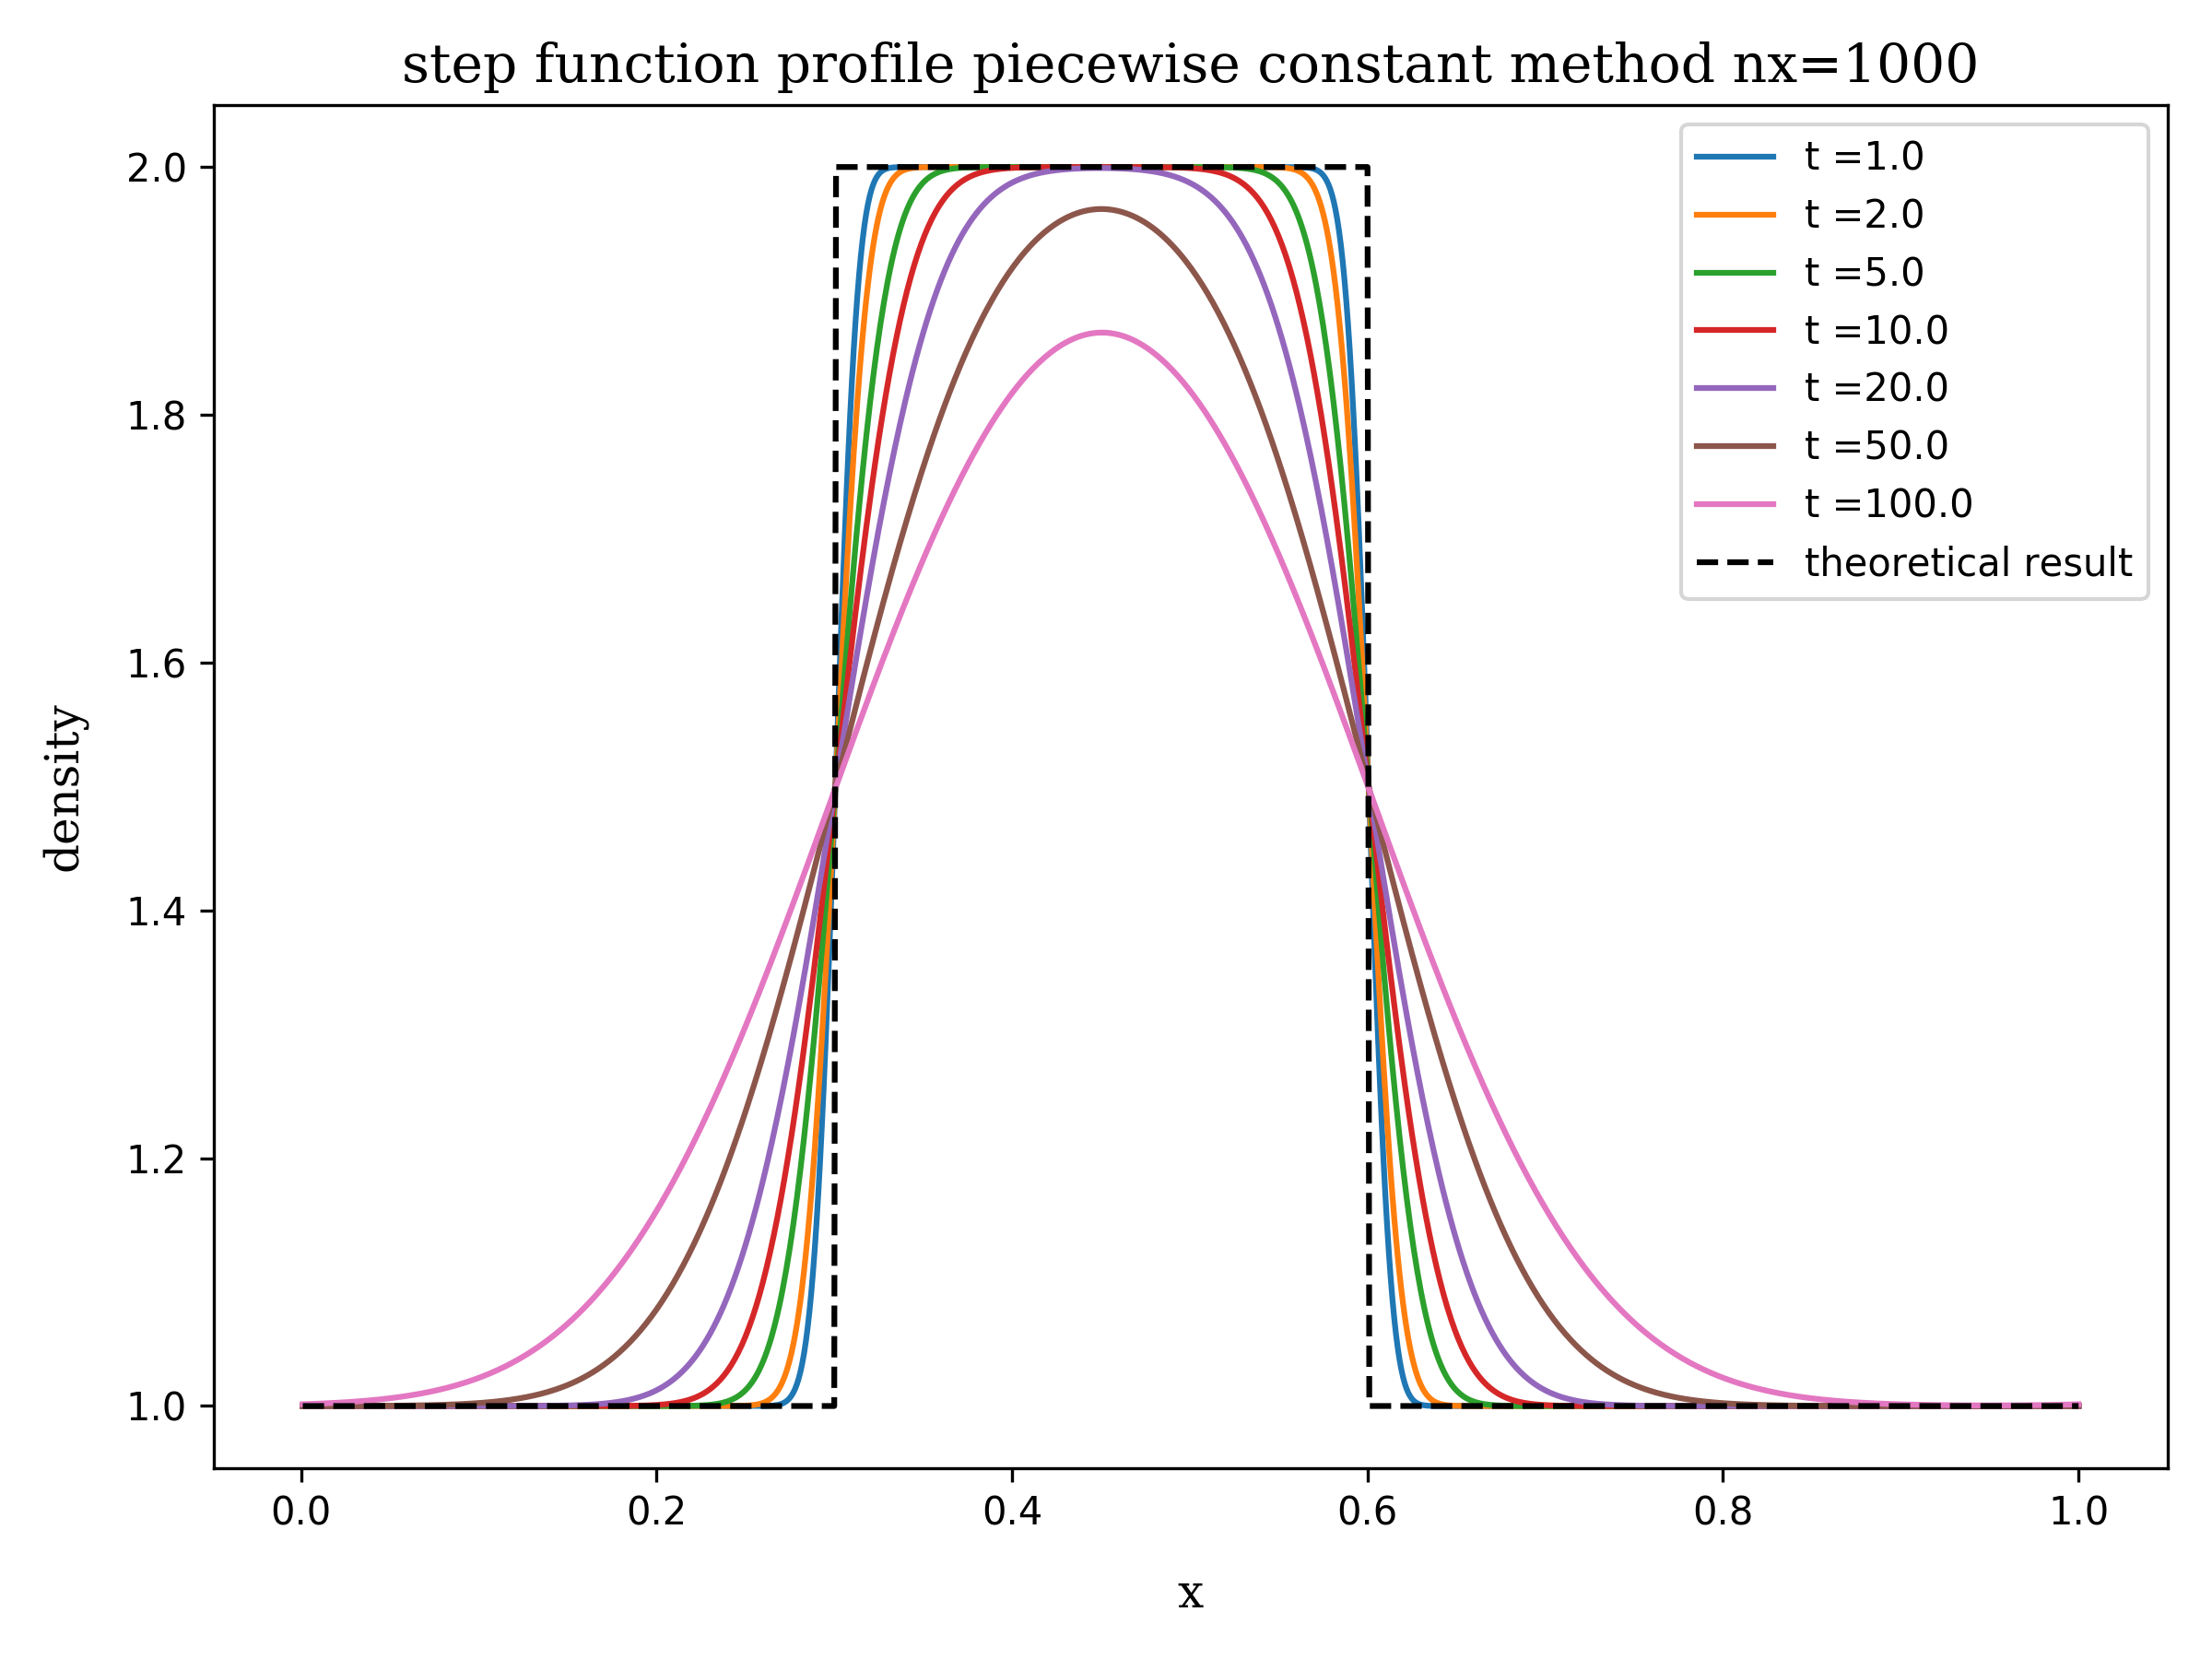
\includegraphics[height=.33\textheight]{../results/1D/pwconst/nx=1000/plot_advection_step_function_pwconst_nx=1000.png}\\
			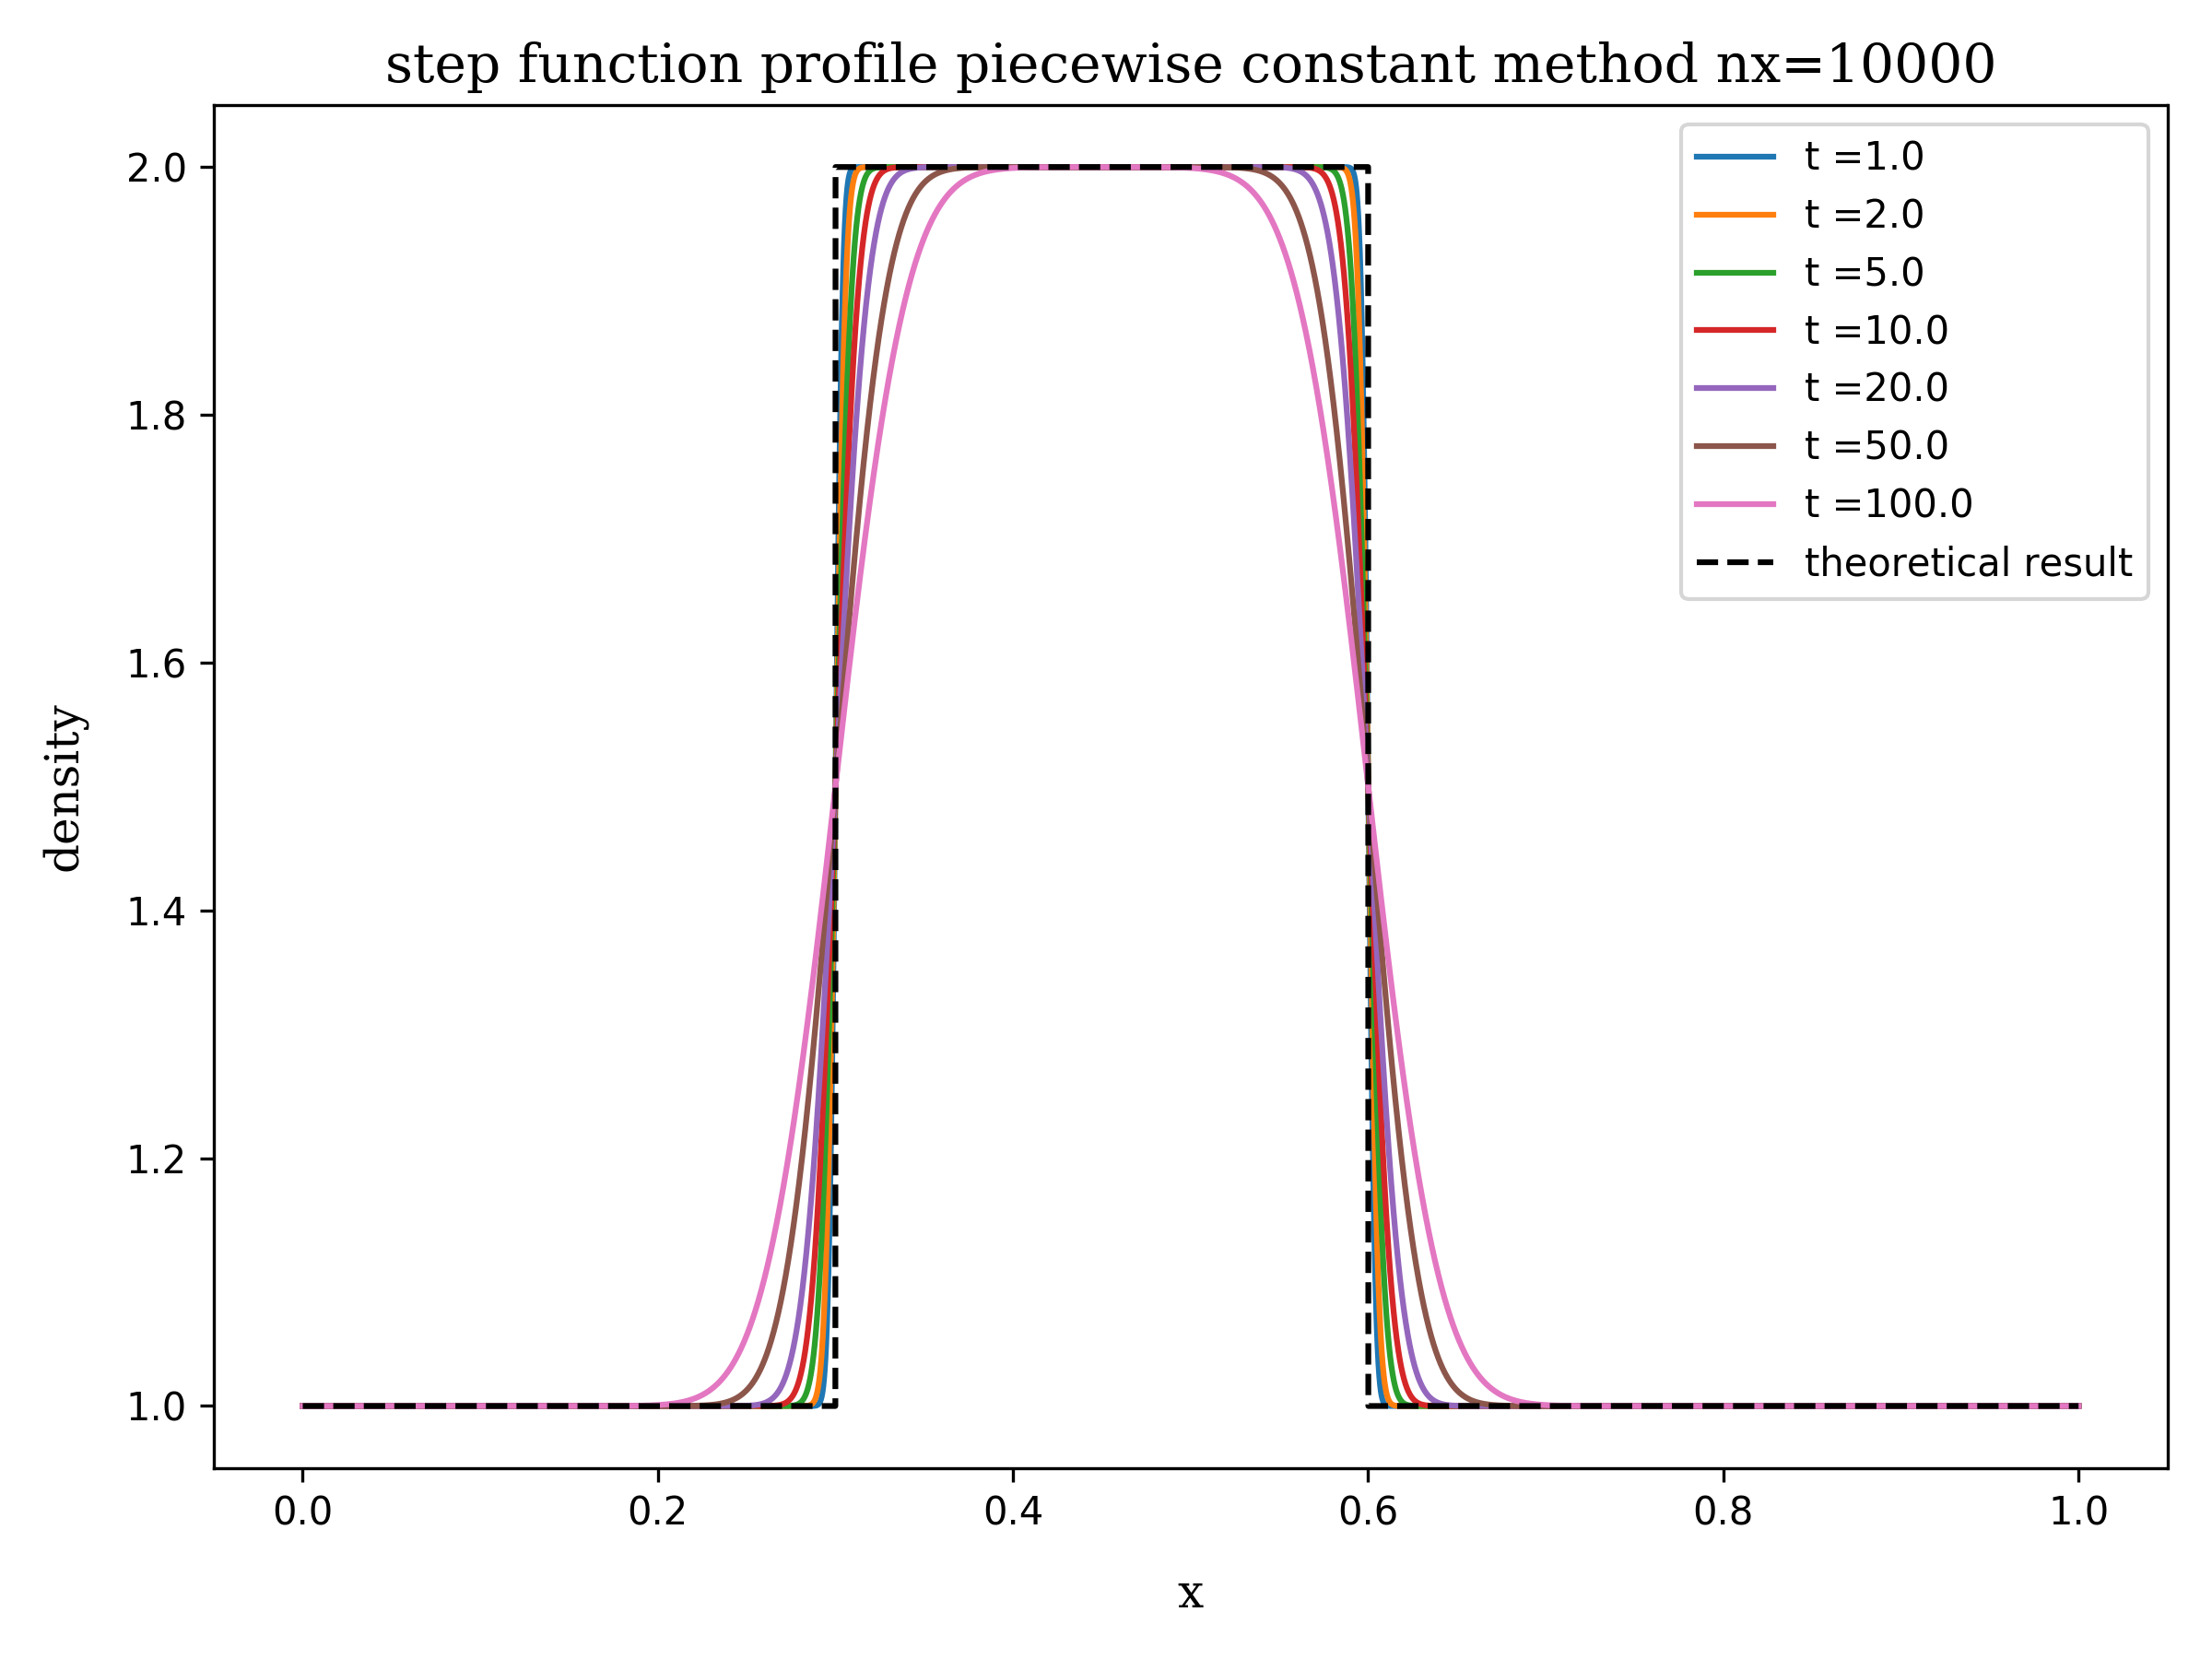
\includegraphics[height=.33\textheight]{../results/1D/pwconst/nx=10000/plot_advection_step_function_pwconst_nx=10000.png}
		\column{.33\textwidth}
			\centering
			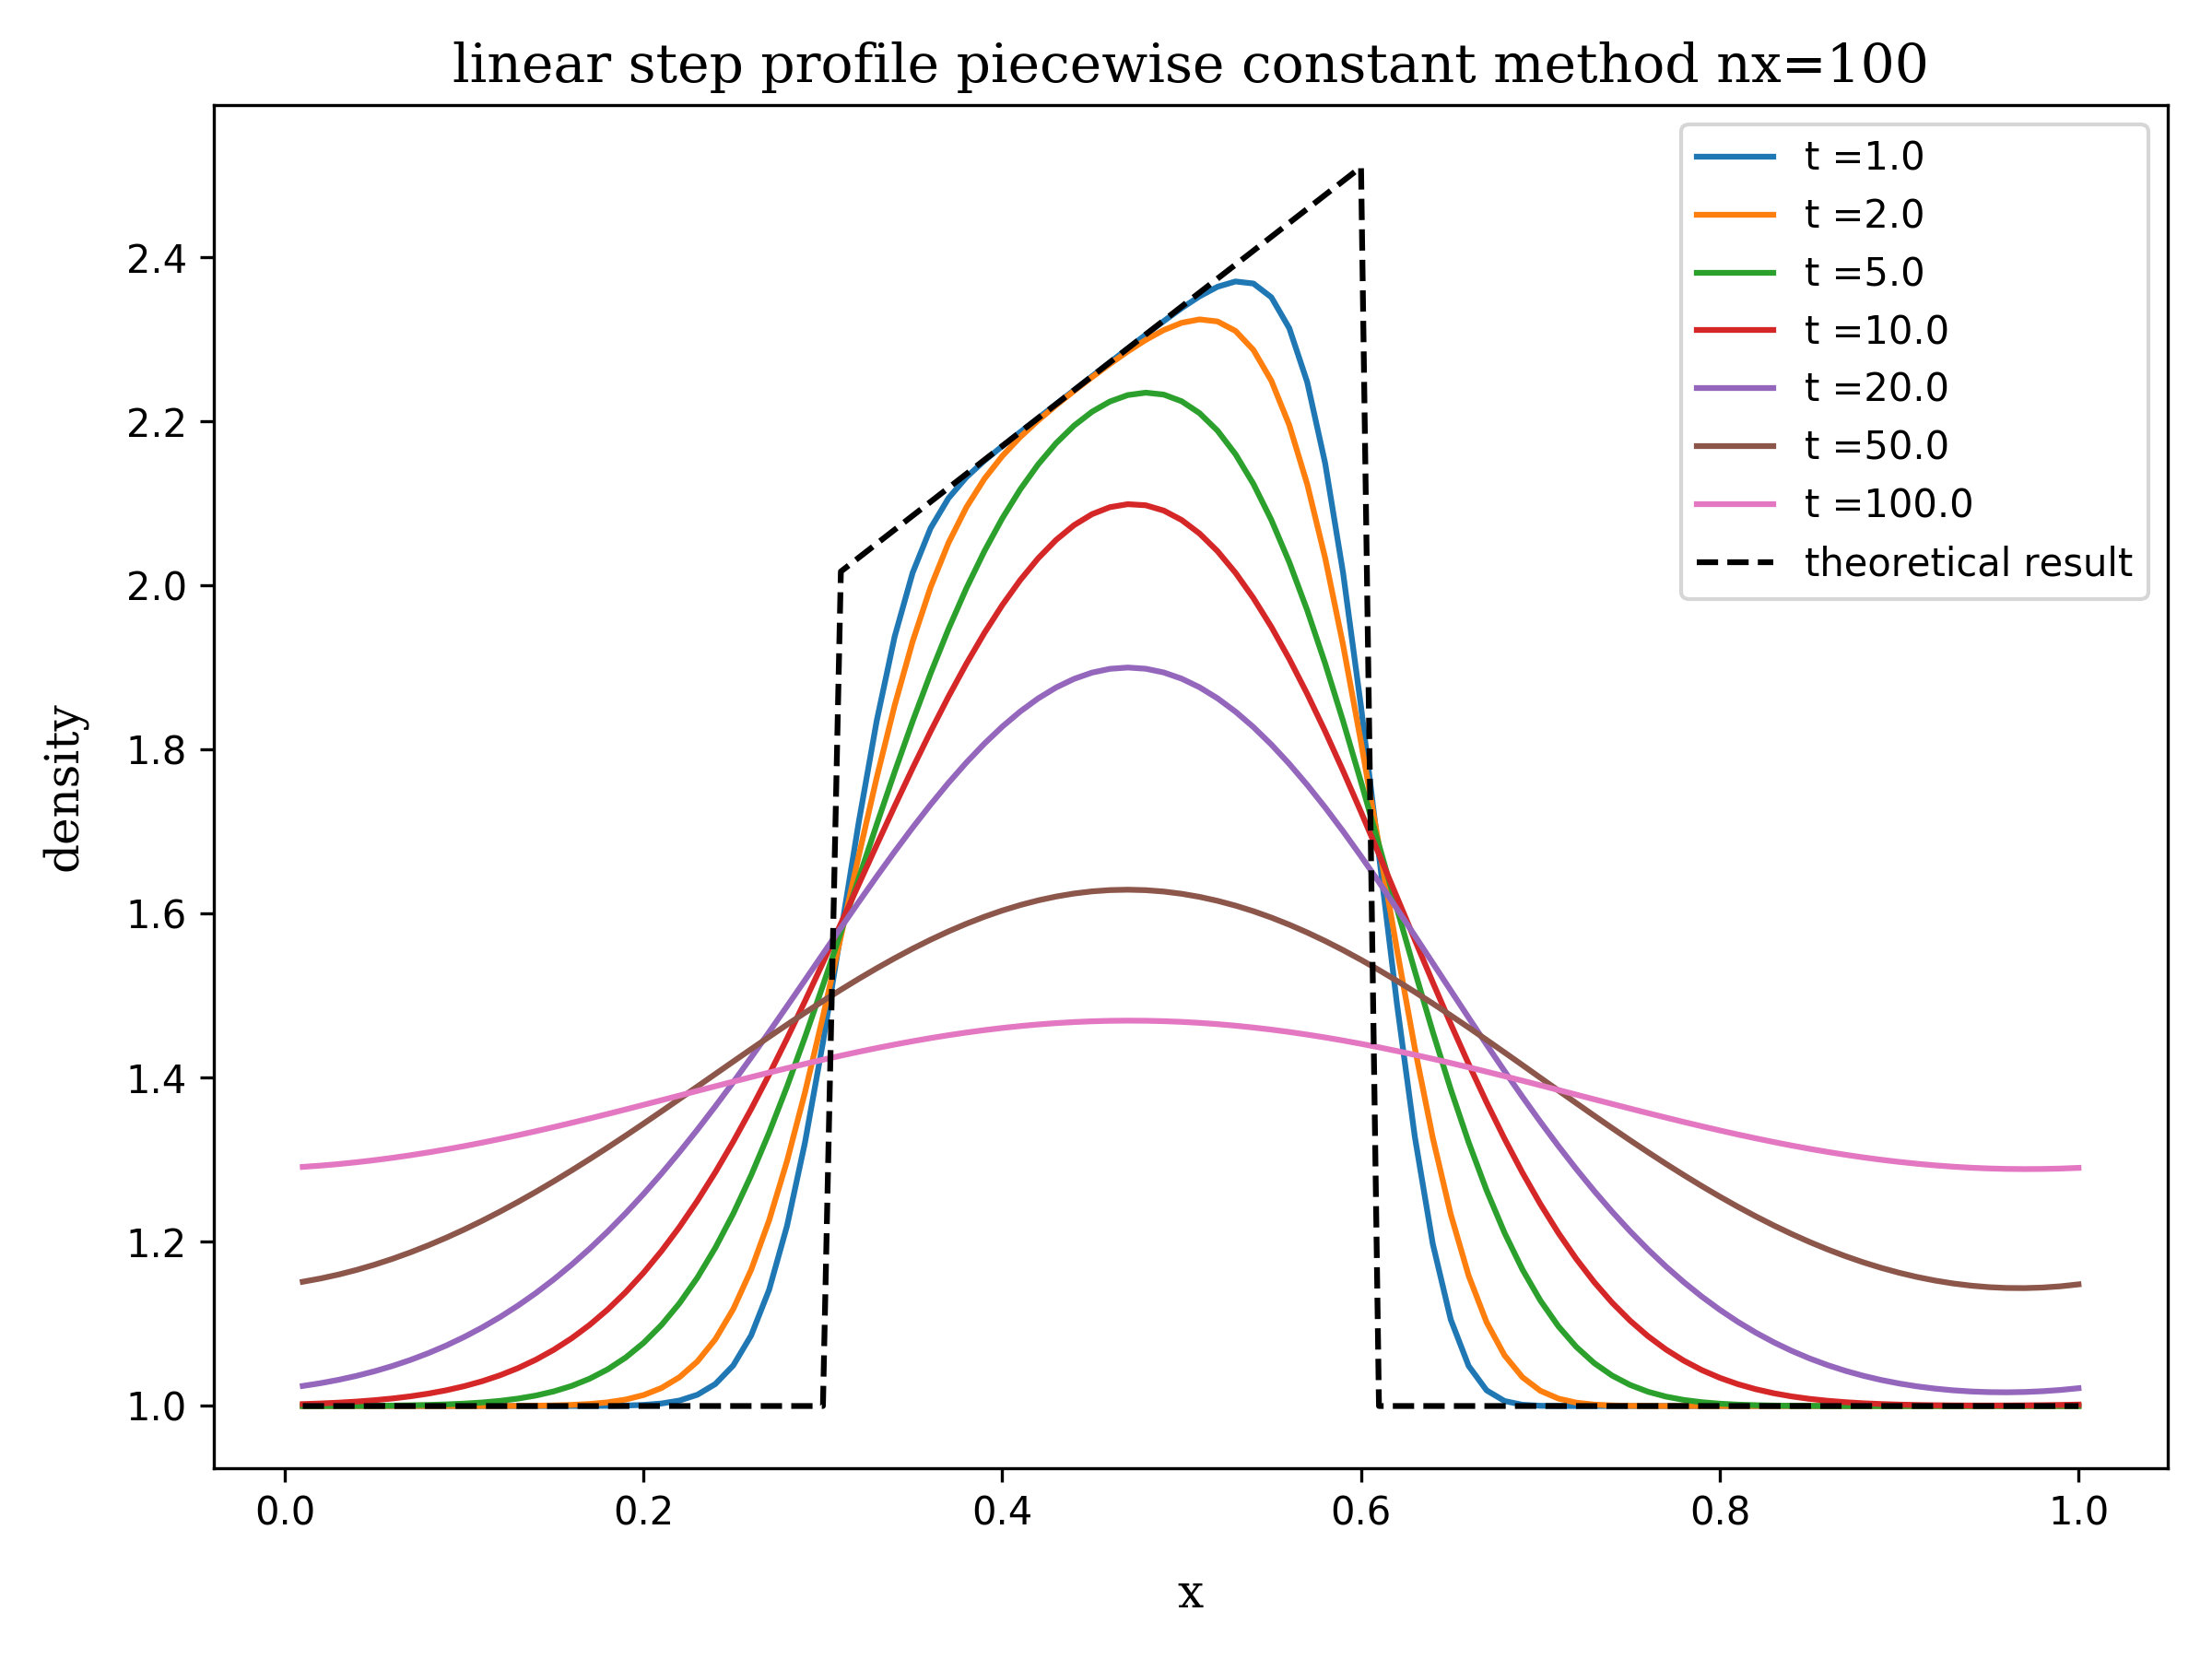
\includegraphics[height=.33\textheight]{../results/1D/pwconst/nx=100/plot_advection_linear_step_pwconst_nx=100.png}\\
			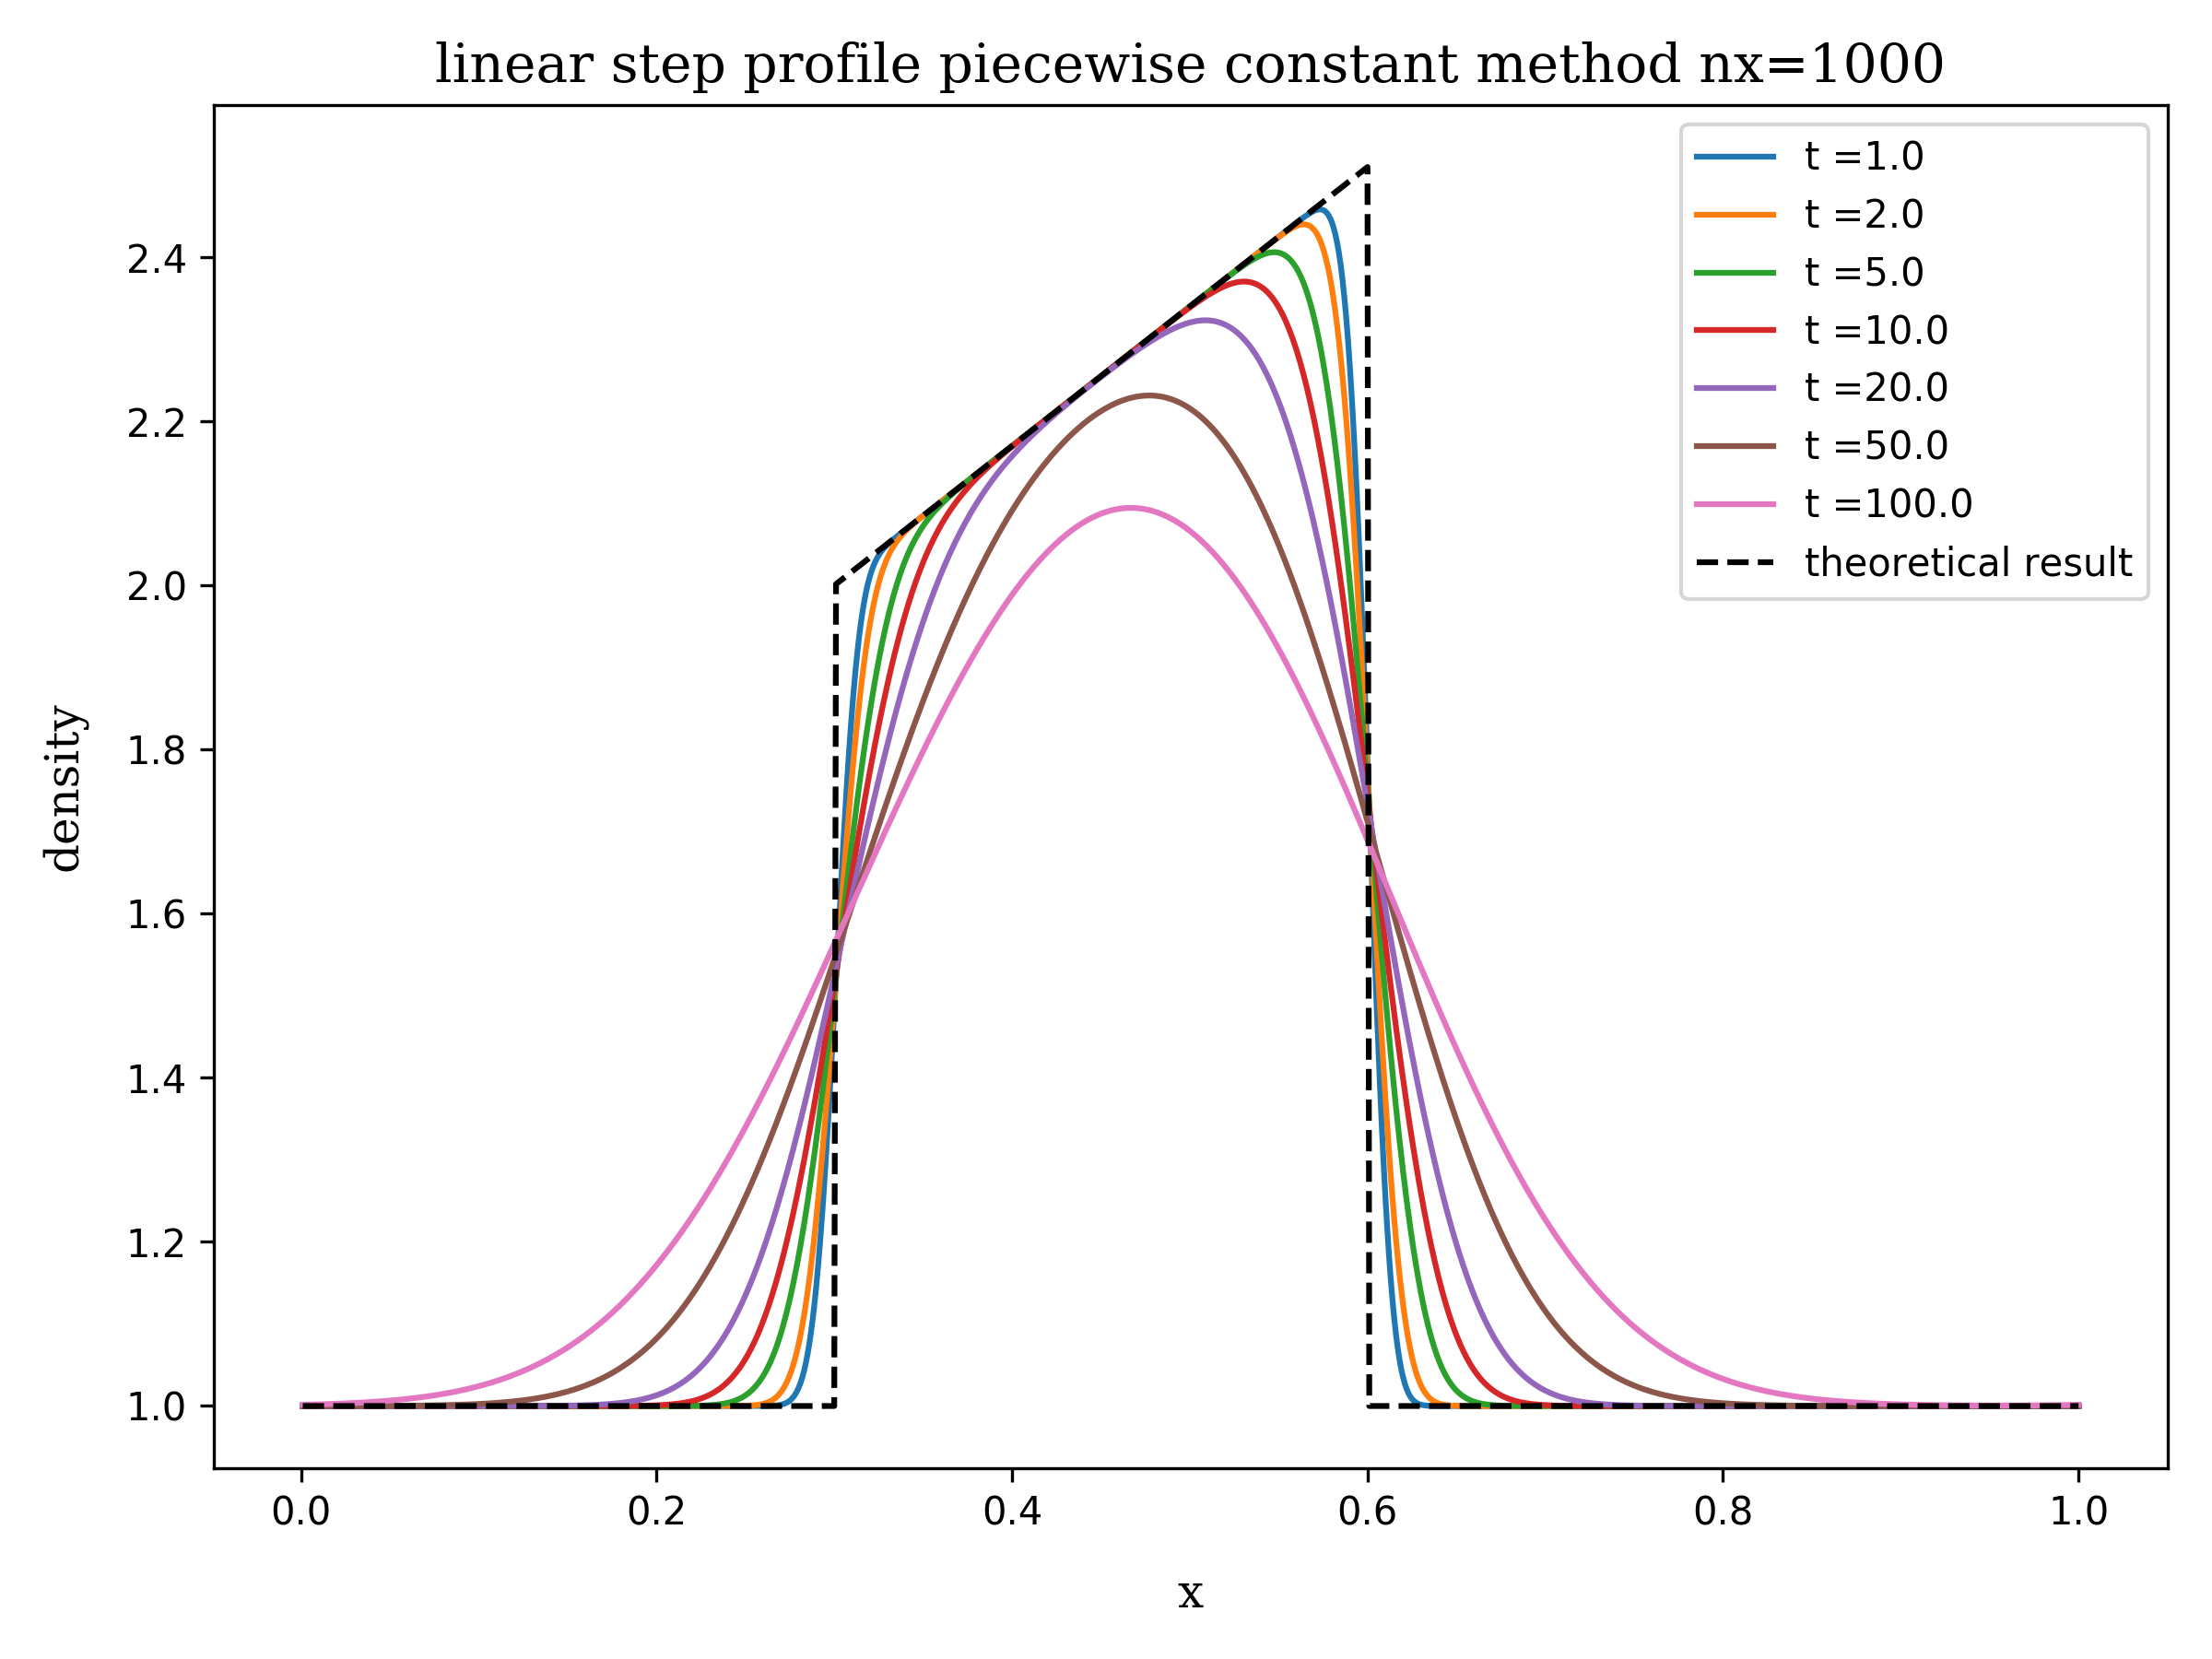
\includegraphics[height=.33\textheight]{../results/1D/pwconst/nx=1000/plot_advection_linear_step_pwconst_nx=1000.png}\\
			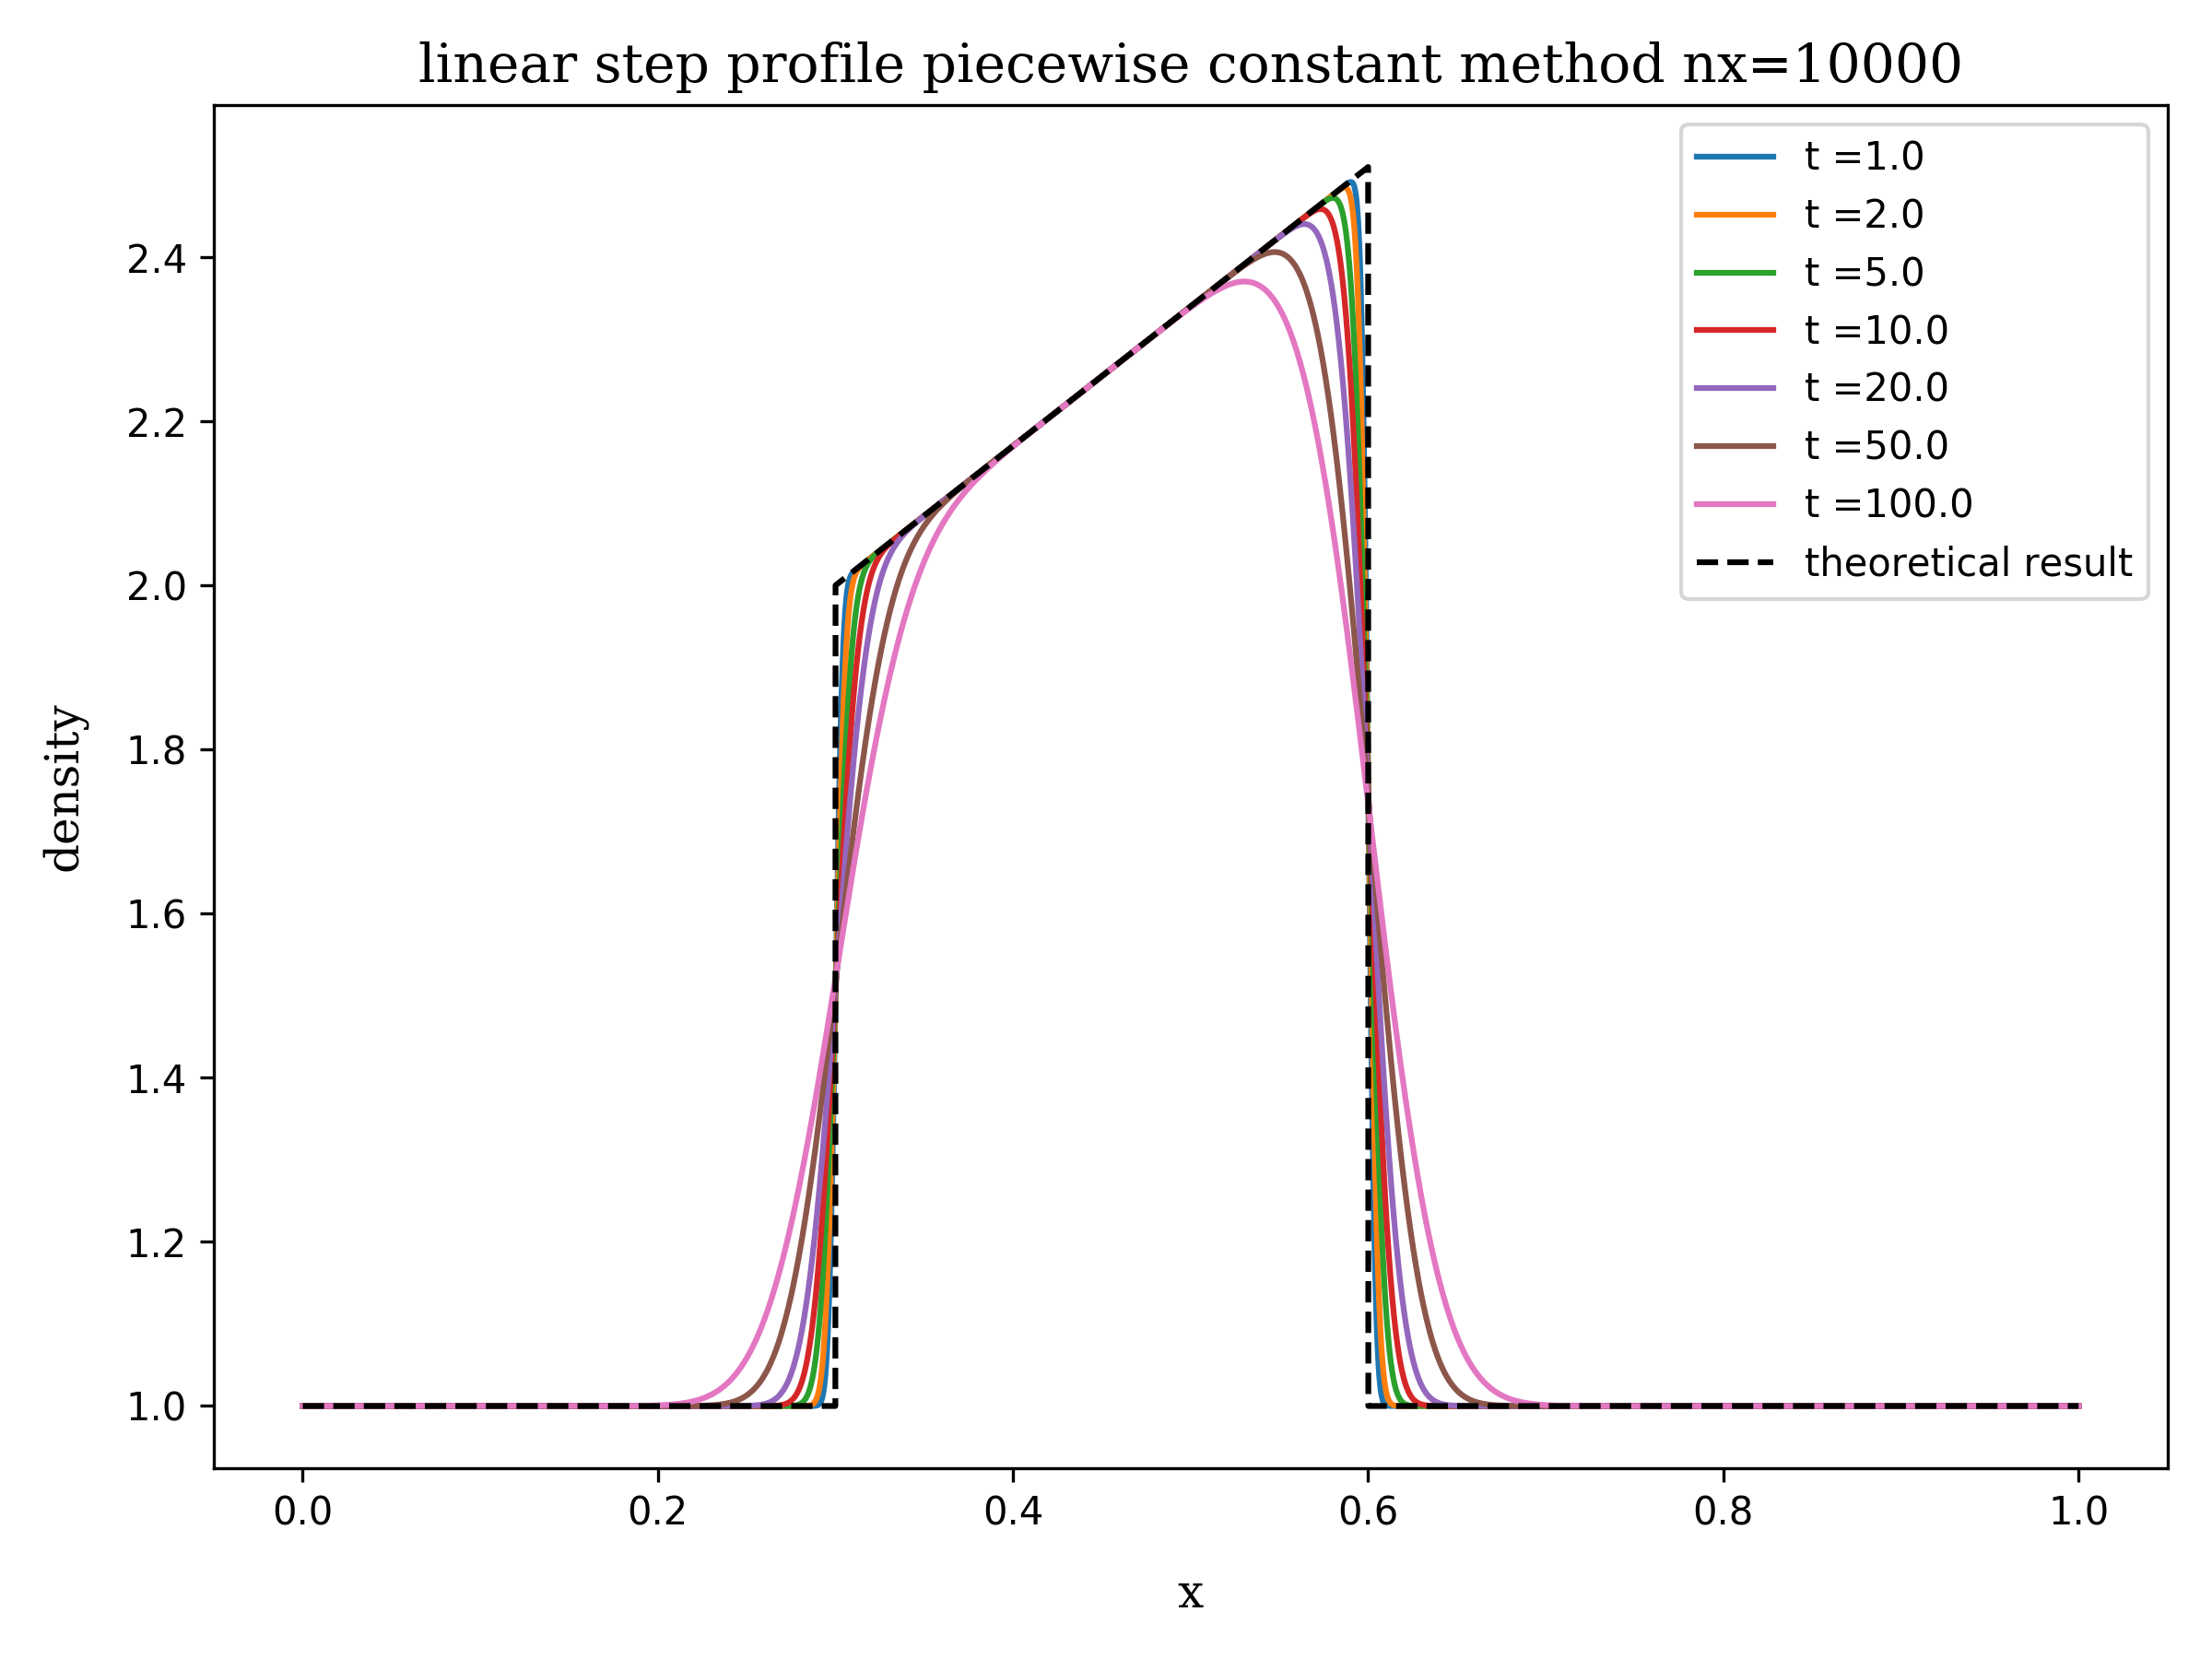
\includegraphics[height=.33\textheight]{../results/1D/pwconst/nx=10000/plot_advection_linear_step_pwconst_nx=10000.png}
		\column{.33\textwidth}
			\centering
			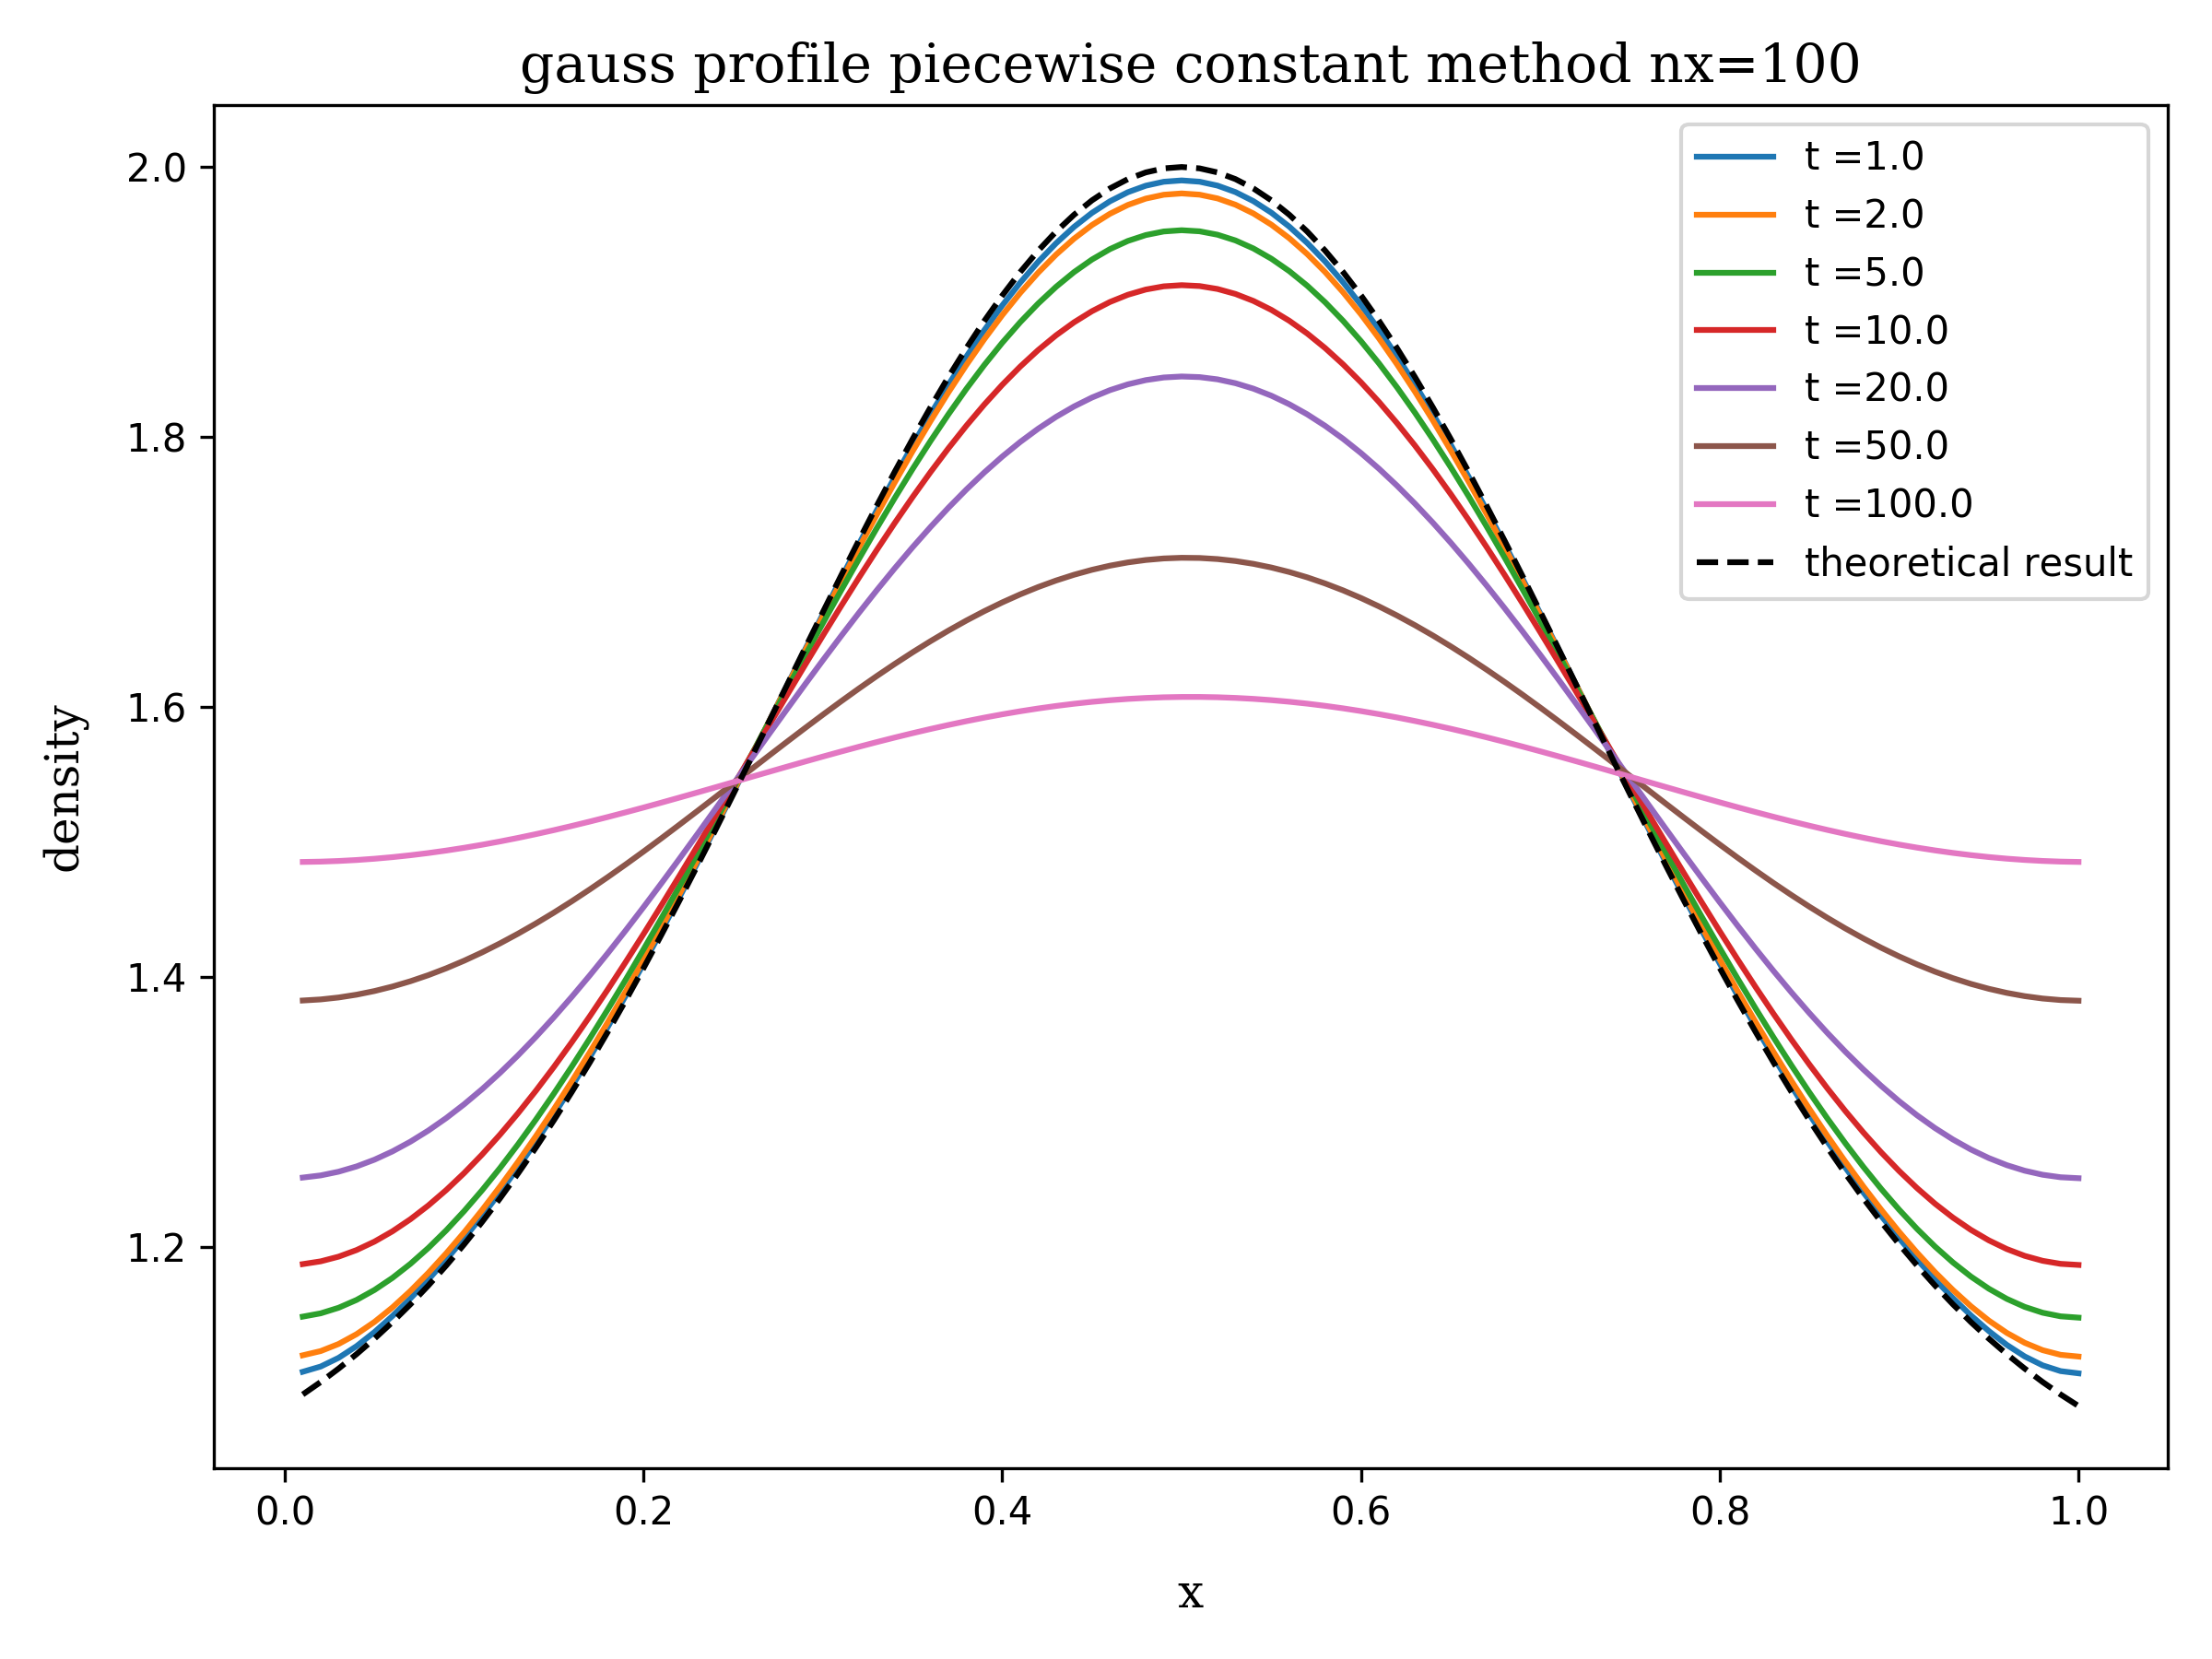
\includegraphics[height=.33\textheight]{../results/1D/pwconst/nx=100/plot_advection_gauss_pwconst_nx=100.png}\\
			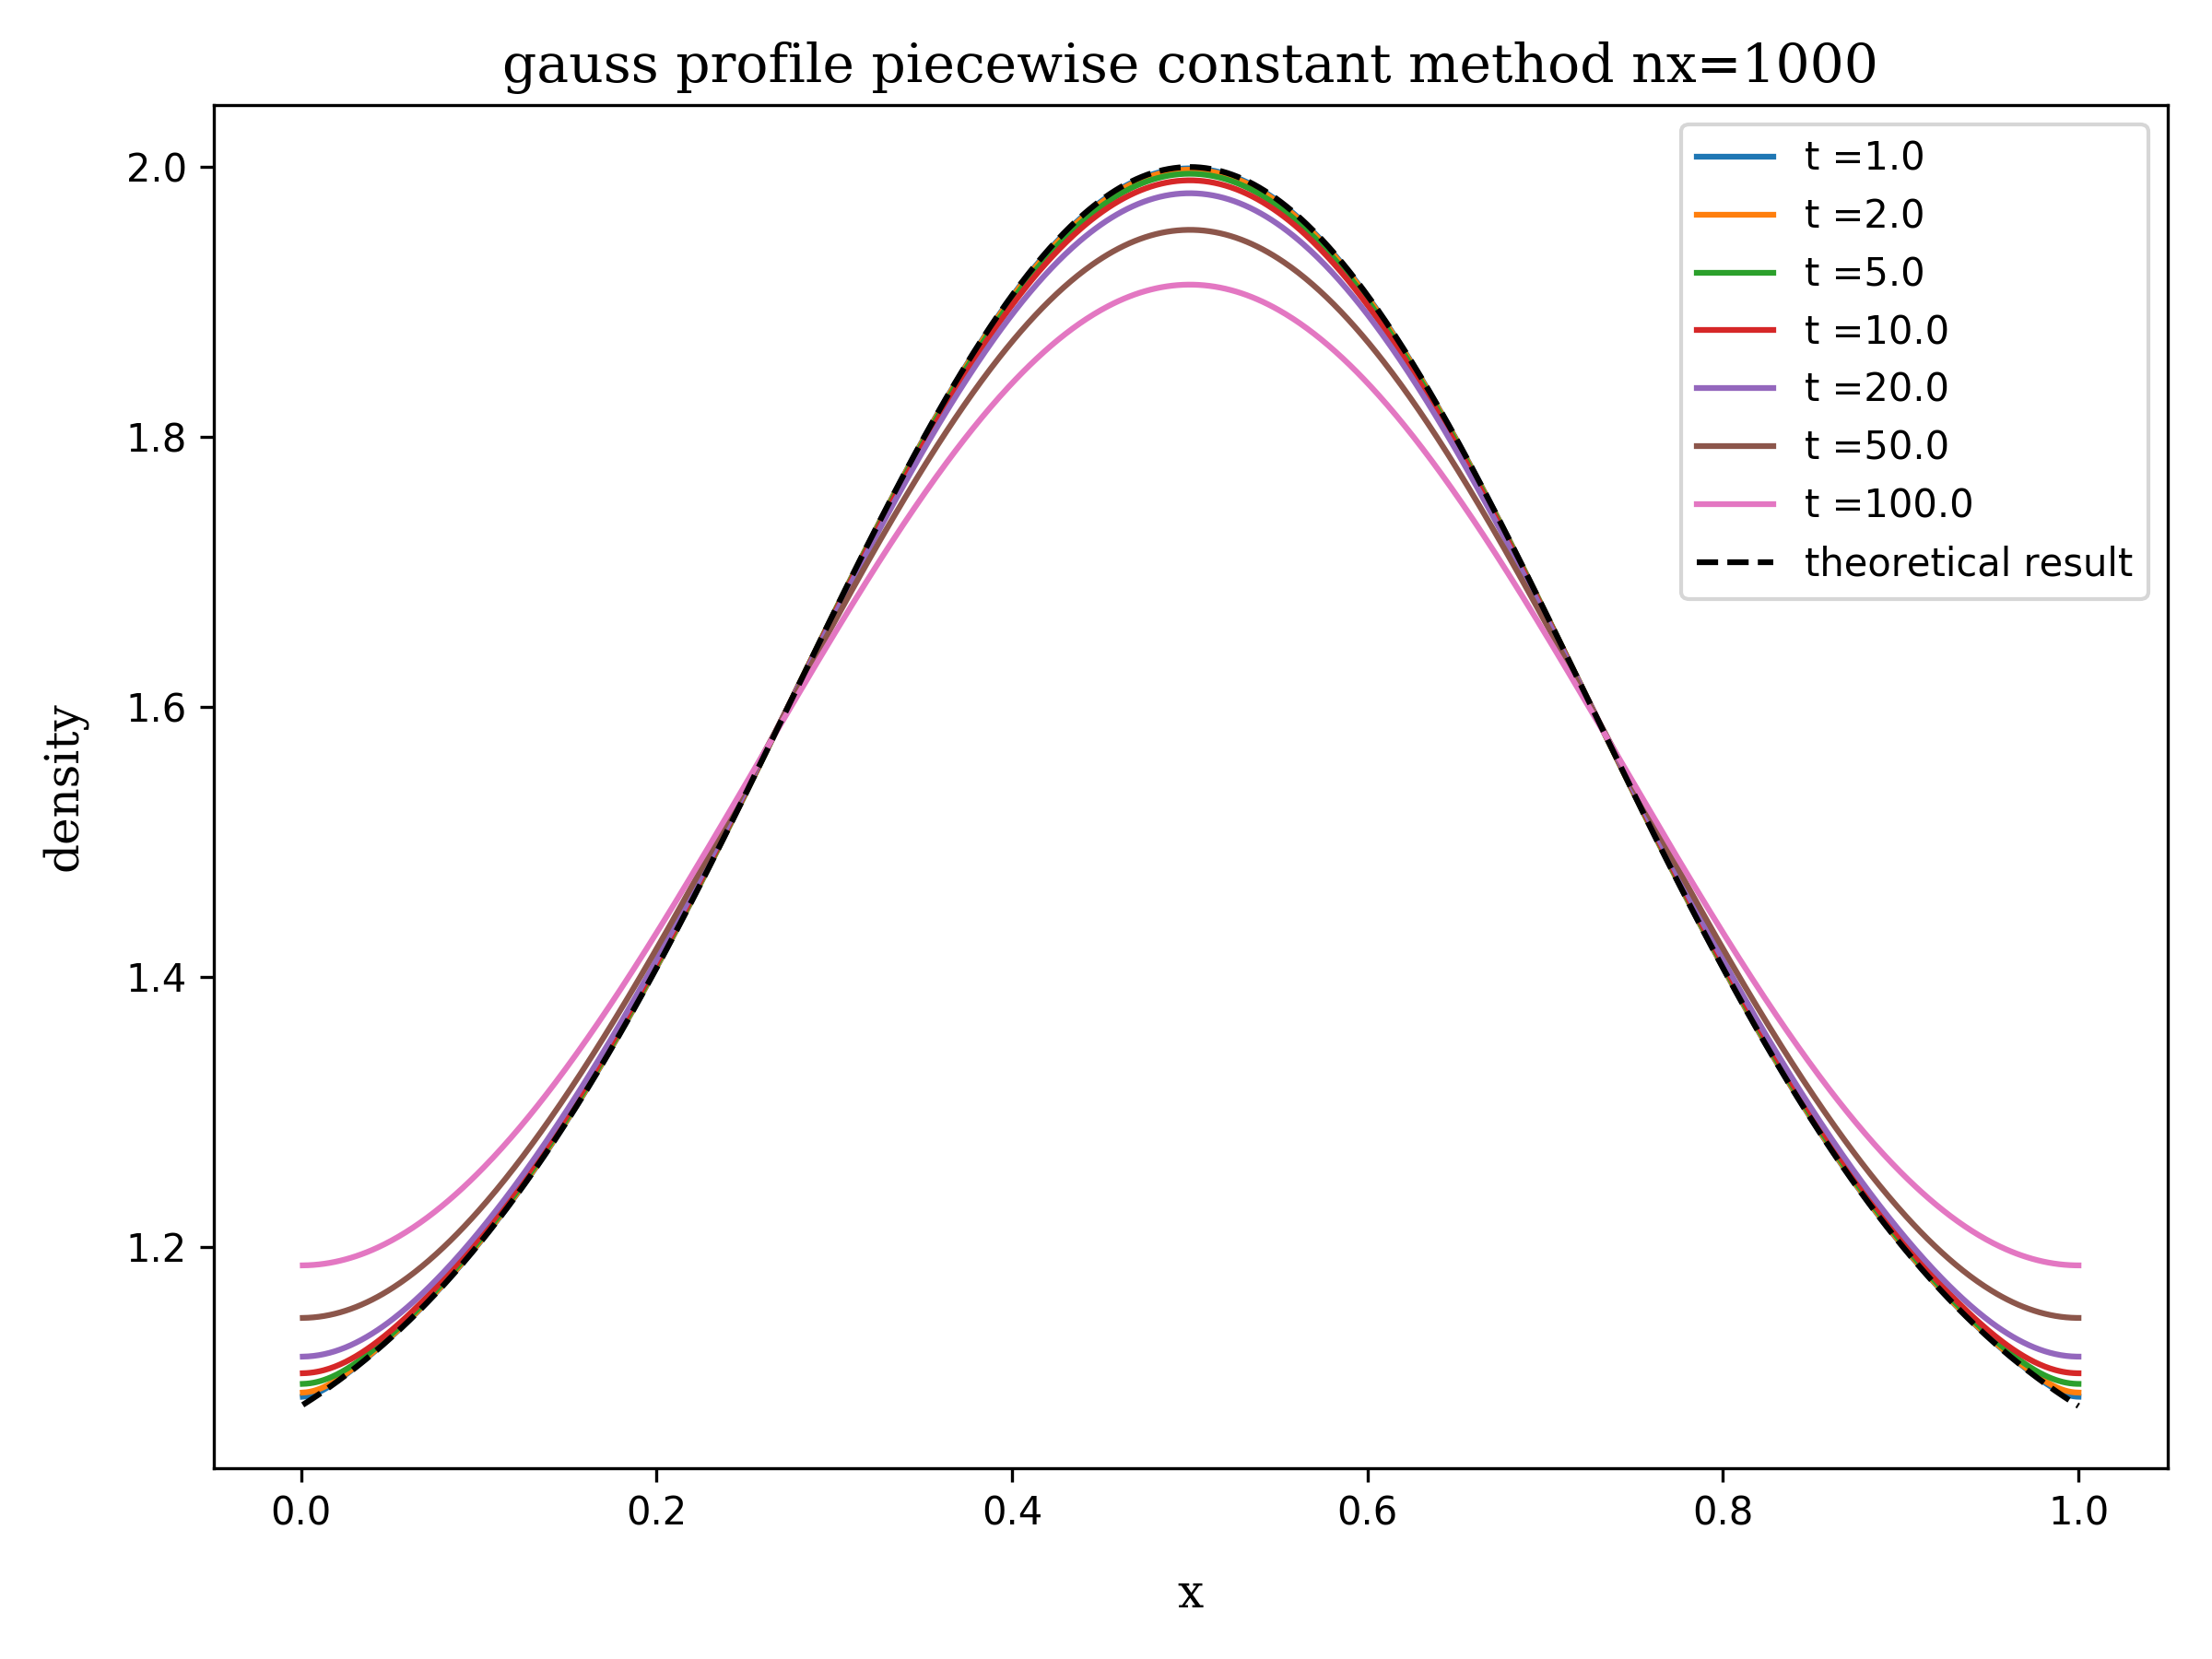
\includegraphics[height=.33\textheight]{../results/1D/pwconst/nx=1000/plot_advection_gauss_pwconst_nx=1000.png}\\
			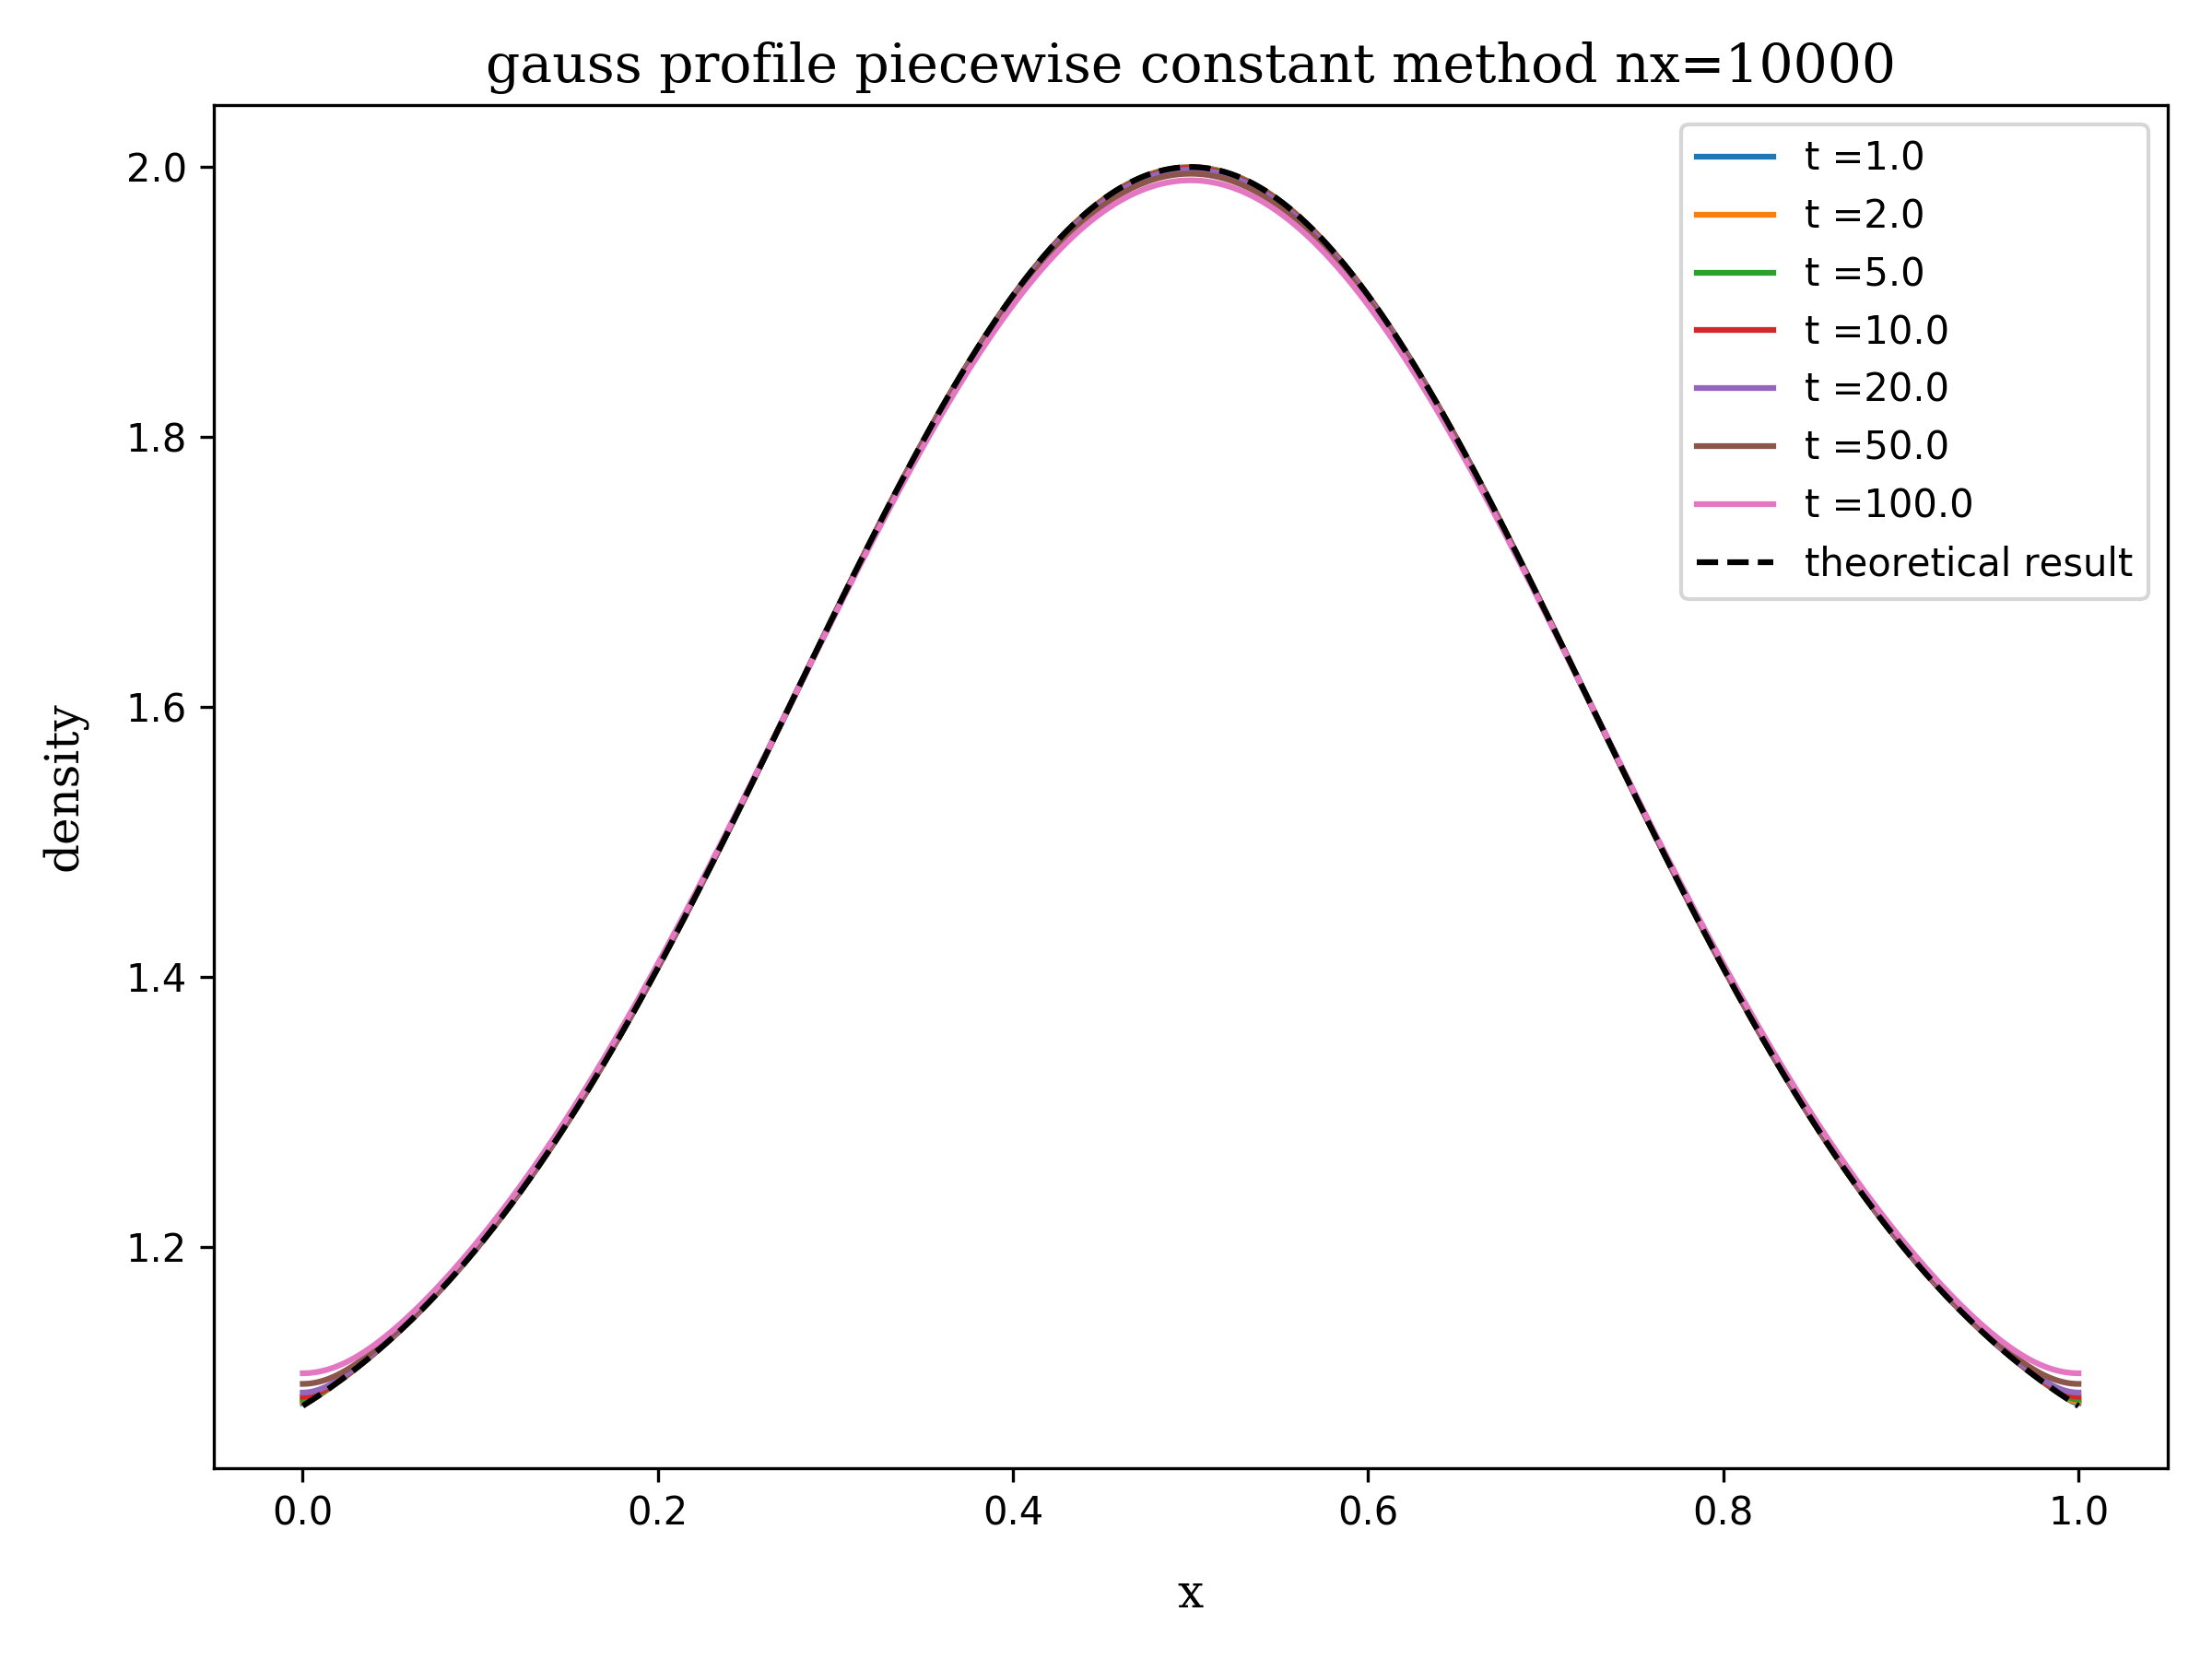
\includegraphics[height=.33\textheight]{../results/1D/pwconst/nx=10000/plot_advection_gauss_pwconst_nx=10000.png}
	\end{columns}
\end{frame}
